\section{Discussion}
\label{sec:bpm2015discuss}

In this section we compare our method to other alternatives for mining data out of logs and interpret our results.

Well known tools that are used in academia and practice include ProM\cite{van2005prom} and Disco\footnote{http://fluxicon.com/disco/}. Both tools require input data to be in the XES~\cite{Verbeek2011} format. Thus, we convert our data from the $\defineExample$ case into XES. To show events per objects of the project structure, we choose the file path as the \emph{caseId}. To flatten the logs we extract all the file paths and build a mapping from each file to the set of changes done to it.

Figure~\ref{fig:dottedchart} depicts the results of the Dotted chart plugin of ProM applied to our log data. Also here, we observe different changes of each file of the repository. While the files and their corresponding events are shown, the plugin does not allow to rearrange the data in order to understand the file structure, nor does it allow to perform any kind of aggregation or connection between data, to observe them from a higher level perspective.

Figure~\ref{fig:discochart} shows the results from mining our log data with the Disco tool. Here we can see a plot that displays the events that happen over time. The plot has some peeks in correspondence to active times of the \emph{example} work package. They can be grouped in three clusters: an initial cluster with a few amount work, an intermediate cluster with the most significant part of the work, and a final cluster that again is not very active. In this way, clusters can be associated to activities. As a drawback, when the number of work packages and activities increase, the number of peeks grows and generate identifying clusters of activities by look at active (or idle) times becomes unworkable.

\begin{figure}
\centering
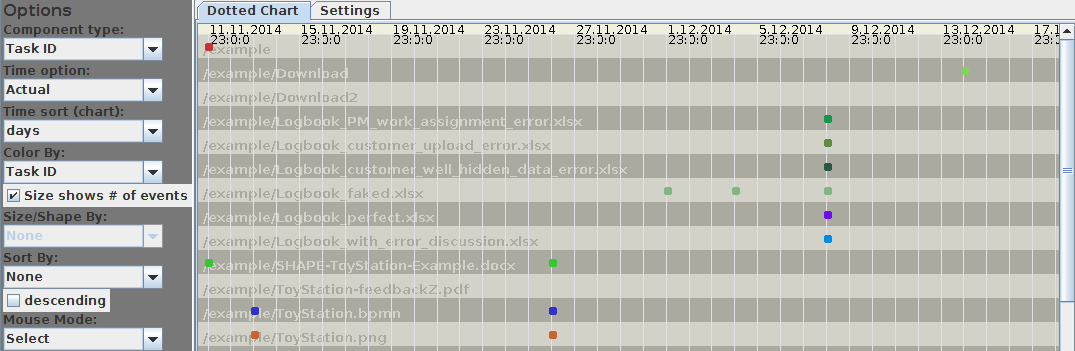
\includegraphics[width=\textwidth]{bpm2015/imgs/dotted_chart_ordered_by_taskID_cut}
\caption{Dotted chart from ProM}
\label{fig:dottedchart}
\end{figure}


\begin{figure}
\centering
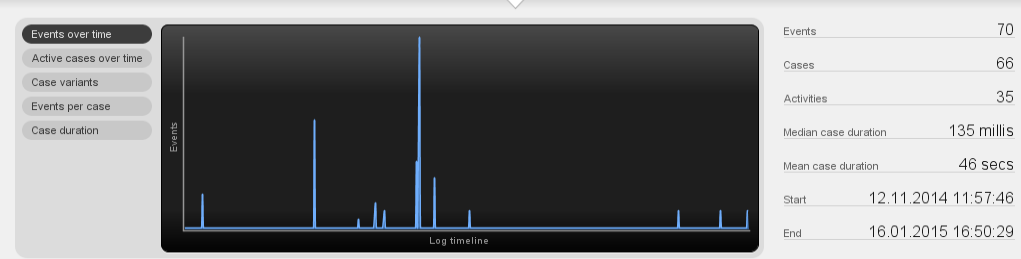
\includegraphics[width=\textwidth]{bpm2015/imgs/disco_screenshot_chart}
\caption{Chart from Disco plotting the events over time.}
\label{fig:discochart}
\end{figure}

Our approach to mining the work progress of project-oriented business processes complements these techniques with metrics and a corresponding visualization that is informative to managers.